\chapter{Diffraction}

Diffraction is what happens when the interference machinery of the previous chapter is pushed to its natural conclusion: instead of two idealized point sources, we allow arbitrarily many, then a continuum. The recurring theme is that every diffraction pattern is the modulus-squared of a Fourier transform of the aperture. Two-slit interference, single-slit diffraction, and the multi-slit grating all fall out as special cases of one formula.

% ============================================================
\section{Multi-Slit Interference}
% ============================================================

Consider $N$ identical narrow slits, spaced by $d$, illuminated by a plane wave and observed at a screen a distance $L \gg Nd$ away. Under this far-field assumption the rays from every slit to the observation point are approximately parallel, so we may take a single observation angle $\theta$ common to all slits, and $\tan\theta \approx \sin\theta \approx y/L$ for small $\theta$.

The geometry is shown in Figure~\ref{fig:multislit-geometry}. Because the screen is far away, the rays leaving adjacent slits toward the observation point are parallel, and the ray from each slit travels an extra distance $d\sin\theta$ relative to its neighbor. The slit-to-slit phase shift is therefore
\begin{equation}
    \delta = \frac{2\pi\, d\sin\theta}{\lambda} \approx \frac{2\pi\, d\, y}{\lambda L}.
\end{equation}
Here $d$ is measured from the center of one slit to the center of the next, not from slit edge to slit edge; this small distinction becomes important once slits acquire finite width.

\begin{figure}[ht]
    \centering
    \begin{tikzpicture}[>=Latex, scale=1.0]
        % barrier with slits
        \def\dsp{1.0}
        \fill[black!20] (-0.15,-2.2) rectangle (0.15,2.2);
        \foreach \k in {-2,-1,0,1,2}{
            \fill[white] (-0.15,{\k*\dsp-0.09}) rectangle (0.15,{\k*\dsp+0.09});
        }
        % incoming plane wave
        \foreach \yy in {-1.8,-1.2,-0.6,0,0.6,1.2,1.8}{
            \draw[blue!55,->] (-1.7,\yy) -- (-0.35,\yy);
        }
        \node[blue!60] at (-1.3,2.15) {\small incoming plane wave};
        % outgoing parallel rays at angle theta
        \def\th{28}
        \foreach \k in {-2,-1,0,1,2}{
            \draw[red!70,->] (0,{\k*\dsp}) -- ++(\th:3.2);
        }
        % two adjacent slits highlighted: path difference triangle
        \coordinate (A) at (0,\dsp);
        \coordinate (B) at (0,0);
        % foot of perpendicular from B onto ray through A
        \draw[dashed] (B) -- ($(A)+(\th-90:{\dsp*sin(\th)})$);
        \coordinate (F) at ($(A)+(\th-90:{\dsp*sin(\th)})$);
        \draw[very thick, blue!60!black] (A) -- (F)
            node[midway, above right=-1pt] {\small $d\sin\theta$};
        % spacing bracket
        \draw[<->] (-0.45,0) -- (-0.45,\dsp) node[midway,left] {\small $d$};
        % angle mark
        \draw[thin] (0.9,0) arc (0:\th:0.9);
        \node at (\th*0.5:1.15) {\small $\theta$};
        \draw[dotted] (0,0) -- (3.0,0);
        % screen
        \draw[very thick] (4.3,-2.3) -- (4.3,2.3);
        \node[rotate=-90] at (4.55,0) {\small screen ($L \gg Nd$)};
    \end{tikzpicture}
    \caption{Far-field geometry for $N$ equally spaced slits. Rays reaching a distant screen at angle $\theta$ are effectively parallel, so each slit's contribution lags its neighbor's by the path difference $d\sin\theta$.}
    \label{fig:multislit-geometry}
\end{figure}

Because $\theta_1\approx\theta_2\approx\cdots\approx\theta$ in the far field, all slits contribute with essentially the same amplitude and wave vector, differing only by the accumulated phase $\delta$ per slit. The total field is then a geometric series:
\begin{equation}
    \vect{E}_{\text{tot}} = \vect{E}_0\, e^{i(\omega t - \vect{k}\cdot\vect{r})} \sum_{m=0}^{N-1} e^{-i m \delta}
    = \vect{E}_0\, e^{i(\omega t - \vect{k}\cdot\vect{r})}\, \frac{1 - e^{-i N \delta}}{1 - e^{-i \delta}}.
\end{equation}
To turn this into something recognizable, factor $e^{-i\delta N/2}$ from the numerator and $e^{-i\delta/2}$ from the denominator; each difference of exponentials then collapses into a sine:
\begin{equation}
    \vect{E}_{\text{tot}} = \vect{E}_0\, e^{i(\omega t - \vect{k}\cdot\vect{r})}\, e^{-i \delta (N-1)/2}\, \frac{\sin(N\delta/2)}{\sin(\delta/2)}.
\end{equation}

The intensity is $\langle I \rangle \propto |E|^2$, and the leftover exponential prefactor (a pure phase) drops out. What remains is the central multi-slit result:
\begin{formula}
\begin{equation}
    \langle I \rangle = I_0 \left[\frac{\sin(N\delta/2)}{\sin(\delta/2)}\right]^2, \qquad \delta = \frac{2\pi\, d\sin\theta}{\lambda}.
\end{equation}
\end{formula}

\subsection{Sanity Checks and Structure}

Before extracting general features, it is reassuring to check that this reduces to something familiar. Setting $N=2$ and using $\sin(\delta) = 2\sin(\delta/2)\cos(\delta/2)$ recovers the two-slit pattern:
\begin{equation}
    \langle I \rangle = I_0\left[\frac{2\sin(\delta/2)\cos(\delta/2)}{\sin(\delta/2)}\right]^2 = 4 I_0 \cos^2(\delta/2),
\end{equation}
as expected.

For $N>2$ the structure of the pattern is richer, but every feature comes directly from the zeros of the numerator and denominator.

\begin{fact}[Structure of the $N$-slit pattern]
For $N > 2$ the intensity exhibits \emph{principal maxima} at $\delta = 2\pi n$ (equivalently $d\sin\theta = n\lambda$), where the numerator and denominator vanish together so that L'H\^opital's rule gives $\langle I\rangle \to N^2 I_0$. Between two consecutive principal maxima the numerator produces $N-1$ minima (zeros not shared with the denominator), and squeezed between those minima are $N-2$ much smaller \emph{secondary maxima} that carry very little of the total power.
\end{fact}

Figure~\ref{fig:nslit-intensity} plots this pattern for $N=6$. The tall principal maxima are pinned to $\delta = 2\pi n$ and reach $N^2 I_0$, while the low ripples between them are the $N-2$ secondary maxima --- so faint that on the scale of the principal peaks they are barely visible.

\begin{figure}[ht]
    \centering
    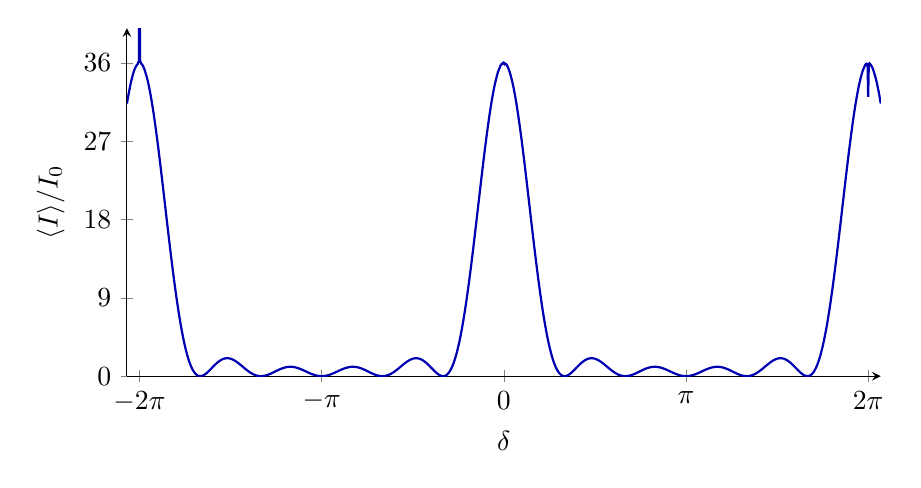
\begin{tikzpicture}
    \begin{axis}[
        width=0.92\textwidth, height=6cm,
        trig format plots=rad,
        xlabel={$\delta$}, ylabel={$\langle I\rangle / I_0$},
        domain=-6.5:6.5, samples=1200,
        xtick={-6.2832,-3.1416,0,3.1416,6.2832},
        xticklabels={$-2\pi$,$-\pi$,$0$,$\pi$,$2\pi$},
        ytick={0,9,18,27,36}, ymin=0, ymax=40,
        enlargelimits=false, clip=true,
        every axis plot/.append style={thick},
        axis lines=left,
    ]
        \addplot[blue!70!black] {(sin(6*x/2)/sin(x/2))^2};
    \end{axis}
    \end{tikzpicture}
    \caption{Six-slit interference intensity as a function of the slit-to-slit phase $\delta$. Principal maxima of height $N^2 I_0 = 36 I_0$ sit at $\delta = 2\pi n$; between each pair lie $N-1 = 5$ zeros and $N-2 = 4$ weak secondary maxima.}
    \label{fig:nslit-intensity}
\end{figure}

The width of a principal maximum is set by the location of the first adjacent minimum, $N\delta/2 = \pm\pi$, giving
\begin{equation}
    \Delta\delta = \frac{4\pi}{N} \propto \frac{1}{N}.
\end{equation}
So more slits gives sharper principal maxima while their \emph{locations} are unchanged. This narrowing-with-$N$ is exactly the Fourier-transform behavior of a longer aperture producing a narrower spot: more slits equals more light through equals a tighter spot on the screen.

\begin{fact}[Two useful bookkeeping facts]
The minima positions $\delta_{\min} = 2\pi n/N$ depend on $N$. The principal maxima positions $\delta_{\max} = 2\pi m$ do \emph{not} depend on $N$. Secondary (modulation) maxima cannot occur where minima occur.
\end{fact}

\begin{example}[Three-slit vs.\ two-slit pattern]
Consider $N=3$ narrow slits with spacing $d$, illuminated by light of wavelength $\lambda$. The intensity is
\begin{equation}
    \langle I \rangle = I_0 \left[\frac{\sin(3\delta/2)}{\sin(\delta/2)}\right]^2.
\end{equation}
The principal maxima at $\delta = 2\pi n$ still sit at $\sin\theta = n\lambda/d$ --- the same angles as for two slits --- but their peak value is $9 I_0$ rather than $4 I_0$. Between adjacent principal maxima there are $N-1 = 2$ zeros (at $\delta/2 = \pi/3$ and $2\pi/3$), and $N-2 = 1$ secondary maximum midway between them. Evaluating at $\delta/2 = \pi/2$ gives
\begin{equation}
    \langle I\rangle_{\text{sec}} = I_0\left[\frac{\sin(3\pi/2)}{\sin(\pi/2)}\right]^2 = I_0,
\end{equation}
about $11\%$ of the principal maximum. Adding just one slit already dramatically shifts intensity into the principal fringes, previewing the resolving power of true gratings.
\end{example}

\begin{example}[Four narrow slits]
Take $N=4$ slits with $a \ll d$ so slits are effectively narrow. Then
\begin{equation}
    I(\theta) = I_0 \left[\frac{\sin(4\delta/2)}{\sin(\delta/2)}\right]^2 = I_0 \left[\frac{\sin(2\delta)}{\sin(\delta/2)}\right]^2, \qquad \delta = \frac{2\pi d \sin\theta}{\lambda}.
\end{equation}
Principal maxima occur where $\sin(\delta/2) = 0$, i.e.\ $\delta = 2\pi n$, which gives $\sin\theta = n\lambda/d$. Minima occur where $\sin(2\delta) = 0$ but $\sin(\delta/2) \ne 0$:
\begin{equation}
    \delta = \frac{m\pi}{2}, \qquad m \ne \text{multiple of }4,
\end{equation}
so $\sin\theta = m\lambda/(4d)$ for $m = 1, 2, 3, 5, 6, 7, \ldots$. Between consecutive principal maxima there are $N-2 = 2$ small secondary maxima. As $\delta/2 \to 0$, $I \to 16 I_0 = N^2 I_0$, four times the two-slit peak.
\end{example}

\begin{example}[Widening the slit spacing: $d \to 3d$]
If the spacing is tripled while keeping the two-slit form, the phase becomes $\delta' = 6\pi d\sin\theta/\lambda$, and
\begin{equation}
    I = 4 I_0 \cos^2(\delta'/2).
\end{equation}
Minima occur where $\cos(3\pi d\sin\theta/\lambda) = 0$, i.e.\ $\sin\theta = (2n-1)\lambda/(6d)$; the sequence $\lambda/6d,\, \lambda/2d,\, 5\lambda/6d,\, 7\lambda/6d,\ldots$. Maxima are at $\sin\theta = m\lambda/(3d)$. Whenever $m$ is a multiple of $3$, these maxima coincide with the original ($d$-spacing) principal maxima --- the two patterns overlap there.
\end{example}

% ============================================================
\section{Single-Slit Diffraction as Infinite-Beam Interference}
% ============================================================

Having pushed $N$ to arbitrary integers, the natural next step is to push it to infinity. A single slit of finite width $a$ can be modeled as an infinite number of infinitesimally narrow slits packed within $|y'| \le a/2$, each with its own slightly different path length. Replacing the discrete sum by an integral,
\begin{equation}
    \vect{E}_{\text{tot}} \propto \int_{-a/2}^{a/2} e^{-i \xi\, y'}\dd y', \qquad \xi \defeq \frac{2\pi \sin\theta}{\lambda}.
\end{equation}
More generally, an aperture with transmission function $S(y')$ gives
\begin{formula}
\begin{equation}
    \vect{E}_{\text{tot}} \propto \int_{-\infty}^{\infty} S(y')\, e^{-i \xi y'}\dd y'.
\end{equation}
\end{formula}
This is exactly the Fourier transform of the aperture function evaluated at spatial frequency $\xi$. Every diffraction pattern is, at heart, a Fourier transform.

Evaluating the integral for the rectangular slit $S(y') = 1$ for $|y'|\le a/2$ and $0$ otherwise,
\begin{equation}
    \vect{E}_{\text{tot}} \propto \frac{1}{-i\xi}\left[e^{-i\xi y'}\right]_{-a/2}^{a/2}
    = \frac{2\sin(a\xi/2)}{\xi}.
\end{equation}
Introducing the dimensionless variable
\begin{equation}
    \beta \defeq \frac{a\, \xi}{2} = \frac{\pi\, a \sin\theta}{\lambda},
\end{equation}
the field amplitude is proportional to $\sin(\beta)/\beta = \operatorname{sinc}(\beta)$, and the intensity becomes
\begin{formula}
\begin{equation}
    \langle I \rangle = I_0\, \frac{\sin^2\beta}{\beta^2}, \qquad \beta = \frac{\pi\, a \sin\theta}{\lambda}.
\end{equation}
\end{formula}

The behavior of this function, plotted in Figure~\ref{fig:sinc}, is worth pausing on. Its zeros sit at $\beta = m\pi$, i.e.\ at $\sin\theta = m\lambda/a$ for nonzero integer $m$, and its central lobe has angular half-width $\lambda/a$ --- so the full central peak spans $2\lambda/a$ between the first zeros.

\begin{figure}[ht]
    \centering
    \begin{tikzpicture}
    \begin{axis}[
        width=0.92\textwidth, height=6cm,
        trig format plots=rad,
        xlabel={$\beta = \pi a\sin\theta/\lambda$}, ylabel={$\langle I\rangle / I_0$},
        domain=-9.6:9.6, samples=600,
        xtick={-9.4248,-6.2832,-3.1416,0,3.1416,6.2832,9.4248},
        xticklabels={$-3\pi$,$-2\pi$,$-\pi$,$0$,$\pi$,$2\pi$,$3\pi$},
        ytick={0,0.25,0.5,0.75,1}, ymin=0, ymax=1.08,
        enlargelimits=false, clip=true,
        axis lines=left,
    ]
        \addplot[thick, red!70!black] {(sin(x)/x)^2};
    \end{axis}
    \end{tikzpicture}
    \caption{Single-slit diffraction intensity $\operatorname{sinc}^2\beta = \sin^2\beta/\beta^2$. The central lobe (between the first zeros at $\beta = \pm\pi$) is twice as wide as the side lobes, whose peak heights fall off as $1/\beta^2$.}
    \label{fig:sinc}
\end{figure} A narrower slit therefore produces a \emph{wider} diffraction pattern, the classic reciprocal relationship characteristic of Fourier transforms. Away from the center the intensity falls off rapidly as $1/\beta^2$, so almost all the diffracted power lives within a few multiples of $\lambda/a$. Although the phenomenon is traditionally called ``diffraction,'' its mechanism is really just interference of infinitely many phase-shifted sources; there is no new physical principle beyond superposition.

\begin{example}[Single-slit central maximum width]
A slit of width $a = 0.10\,\text{mm}$ is illuminated by red light of wavelength $\lambda = 633\,\text{nm}$, and the diffraction pattern is observed on a screen at distance $L = 2.0\,\text{m}$. The first minima occur at $\sin\theta = \lambda/a$, so the full width of the central bright band on the screen is
\begin{equation}
    \Delta y = 2 L \tan\theta \approx 2 L\, \frac{\lambda}{a} = \frac{2 (2.0\,\text{m})(6.33\times 10^{-7}\,\text{m})}{1.0\times 10^{-4}\,\text{m}} \approx 2.5\,\text{cm}.
\end{equation}
Halving the slit width would double this spread --- exactly the reciprocal scaling that any Fourier transform exhibits.
\end{example}

\subsection{Recovering Two-Slit Interference from the Fourier Picture}

The same integral formalism must reproduce the old two-slit result as a check. For two point-like slits at $y' = \pm d/2$, $S(y') = \delta(y' - d/2) + \delta(y' + d/2)$, so
\begin{equation}
    \vect{E}_{\text{tot}} \propto e^{-i\xi d/2} + e^{i\xi d/2} \propto \cos(\xi d/2) = \cos\!\left(\frac{\pi d \sin\theta}{\lambda}\right),
\end{equation}
and hence
\begin{equation}
    \langle I \rangle \propto \cos^2\!\left(\frac{\pi\, d \sin\theta}{\lambda}\right),
\end{equation}
which is precisely the two-slit result. The delta-function slits and the finite-width slits are two ends of the same Fourier-transform machinery.

% ============================================================
\section{Full Multi-Slit Diffraction: Slits with Finite Width}
% ============================================================

Real slits have both a separation $d$ and a nonzero width $a$. The aperture function is a convolution of the two-slit delta comb with a rectangular slit profile, and by the convolution theorem the resulting diffraction pattern is the \emph{product} of the two individual patterns:

\begin{formula}
\begin{equation}
    I(\theta) = I_0 \left(\frac{\sin\beta}{\beta}\right)^2 \cos^2\!\left(\frac{\pi\, d\sin\theta}{\lambda}\right),
\end{equation}
\end{formula}
where $\beta = \pi a \sin\theta/\lambda$ and the second factor equals $\cos^2(\delta/2)$ with $\delta = 2\pi d\sin\theta/\lambda$.

The physical interpretation follows the two length scales in the aperture. Because $a \ll d$ in most experiments, the $\sin^2\beta/\beta^2$ envelope varies slowly with $\theta$ and encodes information about the slit \emph{width}, while the $\cos^2$ factor oscillates rapidly and encodes the slit \emph{spacing}. The peaks of the fast interference pattern are modulated by the slow single-slit envelope, as Figure~\ref{fig:combined} shows, and whenever a two-slit maximum happens to fall at a single-slit minimum, that particular fringe is extinguished --- a ``missing order.''

\begin{figure}[ht]
    \centering
    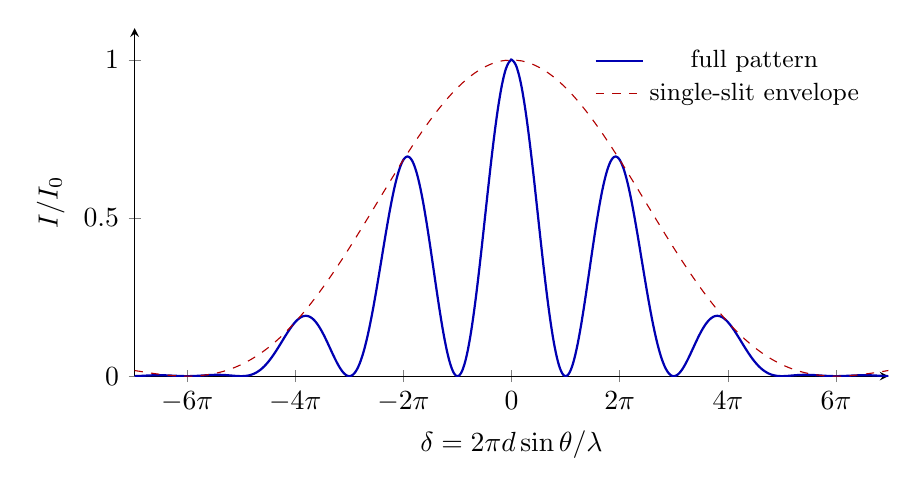
\begin{tikzpicture}
    \begin{axis}[
        width=0.92\textwidth, height=6cm,
        trig format plots=rad,
        xlabel={$\delta = 2\pi d\sin\theta/\lambda$}, ylabel={$I / I_0$},
        domain=-21.9:21.9, samples=1000,
        xtick={-18.85,-12.566,-6.2832,0,6.2832,12.566,18.85},
        xticklabels={$-6\pi$,$-4\pi$,$-2\pi$,$0$,$2\pi$,$4\pi$,$6\pi$},
        ytick={0,0.5,1}, ymin=0, ymax=1.1,
        enlargelimits=false, clip=true,
        axis lines=left,
        legend style={draw=none, fill=none, at={(0.98,0.97)}, anchor=north east, font=\small},
    ]
        \addplot[thick, blue!70!black] {(sin(x/6)/(x/6))^2 * (cos(x/2))^2};
        \addlegendentry{full pattern}
        \addplot[dashed, red!70!black] {(sin(x/6)/(x/6))^2};
        \addlegendentry{single-slit envelope}
    \end{axis}
    \end{tikzpicture}
    \caption{Double-slit pattern with finite slit width ($a = d/3$): the rapid two-slit fringes $\cos^2(\delta/2)$ are modulated by the slow single-slit envelope $\sin^2\beta/\beta^2$ (dashed). The envelope's first zero falls exactly on the third-order fringe ($\delta = 6\pi$), which is therefore a missing order.}
    \label{fig:combined}
\end{figure}

The generalization to $N$ finite-width slits is immediate, since the multi-slit result already handled the delta-comb factor:
\begin{equation}
    I(\theta) = I_0 \left(\frac{\sin\beta}{\beta}\right)^2 \left[\frac{\sin(N\delta/2)}{\sin(\delta/2)}\right]^2,
\end{equation}
again a product of a single-slit envelope and a multi-slit interference factor.

\begin{example}[A missing order]
Consider $D = d/5$ slit width and the intensity pattern
\begin{equation}
    I(\theta) \propto I_0 \left[\frac{\sin(2\delta)}{\sin(\delta)}\right]\left(\frac{\sin\beta}{\beta}\right)^2, \qquad \beta = \frac{D\pi \sin\theta}{\lambda} = \frac{d\pi \sin\theta}{5\lambda}.
\end{equation}
The envelope has minima when $\beta = \ell\pi$, i.e.\ $\sin\theta = 5\ell\lambda/d$. The interference principal maxima sit at $\sin\theta = n\lambda/d$. A principal maximum is extinguished when the two coincide:
\begin{equation}
    \frac{5\ell \lambda}{d} = \frac{n\lambda}{d} \;\Longrightarrow\; n = 5\ell.
\end{equation}
The lowest principal maximum lost is $n = 5$ (with $\ell = 1$): the fifth-order fringe from center is killed by the single-slit envelope. This is the general ``missing orders'' rule for a grating: order $n$ is missing whenever $n/d = \ell/D$.
\end{example}

\begin{example}[Double-slit with finite width]
Two slits of width $a = 0.04\,\text{mm}$ separated by $d = 0.20\,\text{mm}$ are illuminated by $\lambda = 500\,\text{nm}$ light. How many bright interference fringes lie inside the central diffraction envelope? The first envelope zeros sit at $\sin\theta = \pm\lambda/a$, while the interference maxima occur at $\sin\theta = n\lambda/d$. The largest $|n|$ satisfying $|n|\lambda/d < \lambda/a$ is
\begin{equation}
    |n| < \frac{d}{a} = \frac{0.20}{0.04} = 5,
\end{equation}
so orders $n = -4,-3,\ldots,3,4$ are visible: nine bright fringes total inside the central envelope. The orders $n = \pm 5$ are the first missing orders, extinguished exactly at the envelope zeros.
\end{example}

% ============================================================
\section{Fraunhofer Diffraction from an Arbitrary Aperture}
% ============================================================

Collecting the picture: for an aperture with transmission $S(y')$ in the far-field (Fraunhofer) limit, the diffracted field on the screen is
\begin{formula}
\begin{equation}
    \vect{E}_{\text{tot}}(\theta) \propto \int_{-\infty}^{\infty} S(y')\, e^{-i \xi\, y'}\dd y', \qquad \xi = \frac{2\pi\sin\theta}{\lambda},
\end{equation}
\end{formula}
which is (up to overall constants) the Fourier transform $\mathcal{F}[S](\xi)$. The observed intensity is $\langle I\rangle \propto |\mathcal{F}[S](\xi)|^2$.

\begin{theorem}[Diffraction/Fourier correspondence]
Convolution of aperture functions in the object plane becomes multiplication of diffraction patterns on the screen. Two-slit-with-width patterns are the product of the single-slit envelope and the two-slit fringe. Structure on scale $a$ in the aperture produces angular structure on scale $\lambda/a$ on the screen --- the aperture-side and screen-side widths are reciprocal, in exact analogy with the position--momentum uncertainty relation.
\end{theorem}

A striking corollary follows from the linearity of the Fourier transform. If $S(y')$ describes an aperture, its complement is $1 - S(y')$ (a solid barrier with a stopper where the aperture had transmission). Since the Fourier transform of $1$ is $\delta(\xi)$, the complementary field is
\begin{equation}
    \mathcal{F}[1 - S](\xi) = \delta(\xi) - \mathcal{F}[S](\xi),
\end{equation}
so away from $\xi = 0$ the two apertures produce the same diffraction pattern up to sign --- Babinet's principle.

% ============================================================
\section{Diffraction Gratings and Resolution}
% ============================================================

A diffraction grating is just a multi-slit apparatus with $N$ very large. The principal maxima obey the grating equation
\begin{formula}
\begin{equation}
    d\sin\theta_n = n\lambda,
\end{equation}
\end{formula}
so different wavelengths appear at different angles: the grating disperses light into a spectrum, as sketched in Figure~\ref{fig:grating-dispersion}. Because the width of each principal maximum scales as $1/N$, a grating with many rulings produces very sharp spectral lines and thus high wavelength resolution --- the reason gratings replaced prisms in serious spectroscopy.

\begin{figure}[ht]
    \centering
    \begin{tikzpicture}[>=Latex, scale=1.0]
        % grating
        \fill[black!25] (-0.12,-1.9) rectangle (0.12,1.9);
        \foreach \k in {-1.6,-1.2,...,1.6}{
            \fill[white] (-0.12,{\k-0.05}) rectangle (0.12,{\k+0.05});
        }
        \node[align=center] at (0,-2.35) {\small grating};
        % incoming white beam
        \draw[line width=2pt, gray, ->] (-3.2,0) -- (-0.2,0);
        \node[gray] at (-2.4,0.35) {\small white light};
        % zero order (undispersed, straight through)
        \draw[line width=1.5pt, gray, ->] (0.2,0) -- (3.4,0);
        \node[gray] at (3.15,-0.28) {\small $n=0$};
        % first orders: red bends more than blue
        \draw[thick, blue!70!black, ->] (0.15,0.05) -- (22:3.4);
        \draw[thick, green!55!black, ->] (0.13,0.05) -- (30:3.4);
        \draw[thick, red!75!black, ->] (0.1,0.05) -- (38:3.4);
        \node[red!75!black] at (38:3.75) {\small $n=1$};
        \draw[thick, blue!70!black, ->] (0.15,-0.05) -- (-22:3.4);
        \draw[thick, green!55!black, ->] (0.13,-0.05) -- (-30:3.4);
        \draw[thick, red!75!black, ->] (0.1,-0.05) -- (-38:3.4);
        \node[red!75!black] at (-38:3.75) {\small $n=-1$};
    \end{tikzpicture}
    \caption{A grating disperses white light: the zeroth order passes straight through undeviated, while each higher order fans out into a spectrum. Since $\sin\theta_n = n\lambda/d$, longer wavelengths (red) diffract to larger angles than shorter ones (blue).}
    \label{fig:grating-dispersion}
\end{figure}

\begin{fact}[Rayleigh resolution criterion]
Two wavelengths $\lambda$ and $\lambda + \Delta\lambda$ are just resolved at order $n$ when the principal maximum of one falls on the first minimum of the other. Since the principal maximum width in $\delta$ is $2\pi/N$, this gives the resolving power
\begin{equation}
    \frac{\lambda}{\Delta\lambda} = n N.
\end{equation}
More lines and higher order both improve resolution.
\end{fact}

\begin{figure}[ht]
\centering
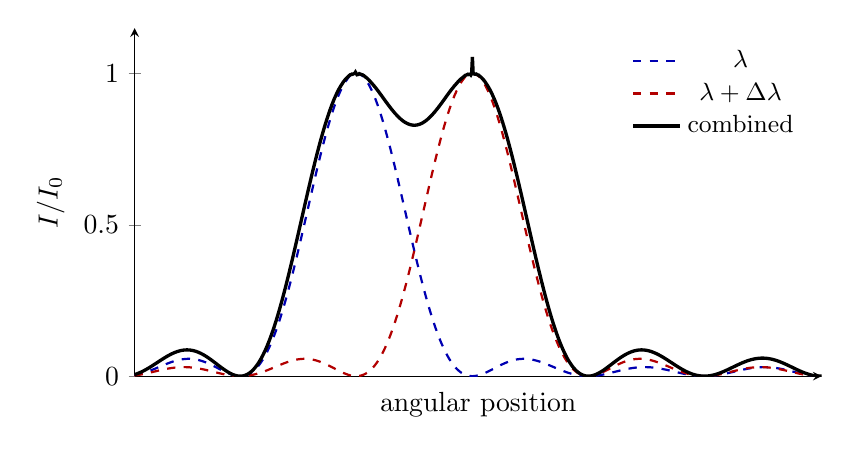
\begin{tikzpicture}
\begin{axis}[
    width=0.85\textwidth, height=6cm,
    trig format plots=rad,
    xlabel={angular position}, ylabel={$I/I_0$},
    domain=-2:4.2, samples=900,
    xtick=\empty,
    ytick={0,0.5,1}, ymin=0, ymax=1.15,
    enlargelimits=false, clip=true,
    axis lines=left,
    legend style={draw=none, fill=none, at={(0.98,0.97)}, anchor=north east, font=\small},
]
    \addplot[dashed, blue!70!black, thick] {(sin(3*x)/sin(x/2+0.0000001))^2/36};
    \addlegendentry{$\lambda$}
    \addplot[dashed, red!70!black, thick] {(sin(3*(x-1.0472))/sin((x-1.0472)/2+0.0000001))^2/36};
    \addlegendentry{$\lambda+\Delta\lambda$}
    \addplot[black, very thick] {(sin(3*x)/sin(x/2+0.0000001))^2/36 + (sin(3*(x-1.0472))/sin((x-1.0472)/2+0.0000001))^2/36};
    \addlegendentry{combined}
\end{axis}
\end{tikzpicture}
\caption{The Rayleigh criterion illustrated with two nearby principal maxima (dashed), each of the $N$-slit shape $[\sin(N\delta/2)/\sin(\delta/2)]^2$ ($N=6$ here), separated by exactly the resolution limit $\Delta\delta = 2\pi/N$ --- the principal maximum of one sits on the first minimum of the other. The combined intensity actually observed (solid) still shows a shallow dip between the two peaks: this is the threshold at which the two wavelengths (or two point sources, in the imaging version of the same criterion) are ``just resolved.'' Any closer and the dip disappears into a single unresolved peak.}
\label{fig:rayleigh}
\end{figure}

The overall angular envelope $\sin^2\beta/\beta^2$ set by the individual slit width still modulates the intensities of the grating orders, so orders that fall near envelope zeros are dim or absent; this is why grating designs often shape the slit profile (blazing) to push power into a desired order.

\begin{example}[Resolving the sodium doublet]
The sodium D lines sit at $\lambda_1 = 589.00\,\text{nm}$ and $\lambda_2 = 589.59\,\text{nm}$, so $\Delta\lambda = 0.59\,\text{nm}$ and
\begin{equation}
    \frac{\lambda}{\Delta\lambda} \approx \frac{589}{0.59} \approx 1000.
\end{equation}
At first order ($n=1$) the grating must therefore have at least $N \gtrsim 1000$ illuminated rulings to just resolve the two lines. A grating ruled at $600\,\text{lines/mm}$ meets this criterion with only $\sim 2\,\text{mm}$ of illuminated width, which is why even modest tabletop spectrometers reveal the doublet clearly.
\end{example}

\begin{example}[Grating angular positions]
A grating with $500\,\text{lines/mm}$ (so $d = 2.0\,\mu\text{m}$) is illuminated at normal incidence by $\lambda = 500\,\text{nm}$ light. The order-$n$ principal maxima appear at
\begin{equation}
    \sin\theta_n = \frac{n\lambda}{d} = \frac{n (500\,\text{nm})}{2000\,\text{nm}} = 0.25\, n.
\end{equation}
Orders $n = 1,2,3$ give $\theta \approx 14.5^\circ,\, 30.0^\circ,\, 48.6^\circ$; the equation fails for $n \ge 5$ since $|\sin\theta|\le 1$, so only four orders on each side of center exist. This finite number of observable orders is a general feature of the grating equation and directly limits the highest order (and hence the resolving power $nN$) achievable for a given $d/\lambda$.
\end{example}

% ============================================================
\section{Summary}
% ============================================================

\begin{fact}[The one formula]
For an arbitrary far-field aperture $S(y')$,
\begin{equation}
    \langle I(\theta)\rangle \propto \left|\int_{-\infty}^{\infty} S(y')\, e^{-i \xi y'}\dd y'\right|^2, \qquad \xi = \frac{2\pi\sin\theta}{\lambda}.
\end{equation}
Every result in this chapter is a special case. A delta-pair $S = \delta(y'-d/2) + \delta(y'+d/2)$ gives the two-slit $\cos^2$ pattern; a rectangle $S = \operatorname{rect}(y'/a)$ gives the single-slit $\operatorname{sinc}^2$ pattern; a delta comb $S = \sum_{m=0}^{N-1} \delta(y' - m d)$ gives the $N$-slit $[\sin(N\delta/2)/\sin(\delta/2)]^2$ pattern; and convolutions in $y'$ become products of patterns in $\theta$.
\end{fact}

The unifying lesson: diffraction is not a separate phenomenon from interference. It is interference of a continuum of coherent sources, and its mathematical content is Fourier analysis of the aperture.
